\section{Introdução}

A teoria de autômatos trata do estudo de máquinas abstratas que seguem
instruções pré-determinadas automaticamente.

<falar sobre níveis da hierarquia de chomsky>

A partir da hierarquia de Chomsky de gramáticas formais, é possível definir
autômatos que são capazes de reconhecer linguagens formais pertencentes a
distintas classes de gramática. Sendo assim, para uma linguagem formal
possivelmente infinita, define-se um autômato como uma representação finita
desta linguagem.

\begin{figure}[H]
    \centering
    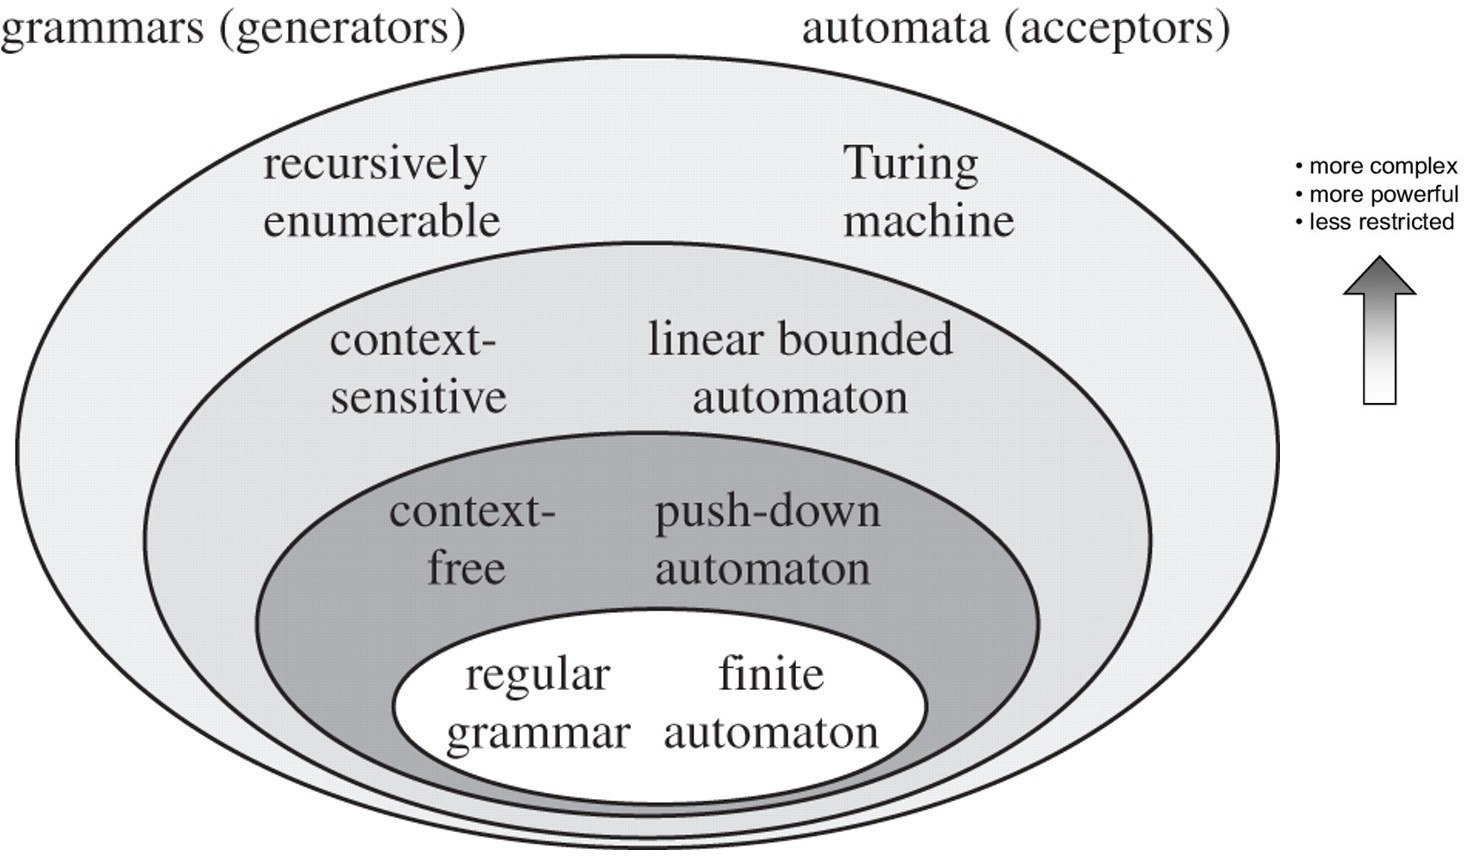
\includegraphics[width=0.8\textwidth]{chomsky}
    \label{chomsky}
    \caption{Hierarquia de Chomsky}
\end{figure}

Dentre os tipos de autômatos existentes, neste trabalho iremos abordar a
construção e o funcionamento das \emph{máquinas de estado finito} e das
\emph{máquinas de Turing}. Estes são responsáveis pelo reconhecimento das
\emph{gramáticas regulares } e \emph{recusivamente enumeráveis},
respectivamente.
